\chapter{Preparation}

\textit{A major part of this project involved reading and understanding the theory behind the models before implementing them. This theory
is described here and so there is overlap with the Implementation chapter, which contains more concrete details on model implementations. 
This chapter also contains information about the success 
criteria and resources used in the project.}

\section{Neural networks}

This project involves using \textbf{autoencoders} as a basis for semi-supervised learning. 
Autoencoder architectures are all based on \textbf{neural networks} so it is important to understand the basic principles.

\subsection{The perceptron}

The perceptron (or \textbf{artificial neuron}) is the basic element of the neural network. It takes in inputs $(x_1, ..., x_n)$ and 
multiplies these by \textbf{weights} $(w_1, ..., w_n)$, giving a linear combination of the inputs $x_1w_1 + ... + x_nw_n$, before applying 
an \textbf{activation function} $\sigma$~\cite{Art_Int}.

It is helpful to think of the inputs and weights as 
vectors $\vec{x}$ and $\vec{w}$, giving the combination as $\vec{x} \cdot \ \vec{w}$. A \textbf{bias} term $x_0=1$ may also be included and multiplied by 
weight $w_0$, giving $\vec{x} = [1, x_1, ..., x_n]$ and $\vec{w} = [w_0, w_1, ..., w_n]$. The bias can be thought of as the intercept
on a graph - if the neuron should have an output when all the inputs are zero it will be unable to model this correctly without a bias.

The function computed by the neuron is then:
\begin{equation}
  y = \sigma(\vec{x} \cdot \vec{w})
\end{equation}

The activation function applied will depend on what the neuron is being used for.
The main activation function used in this project is ReLU, which has the form:
\begin{align}
  \sigma(z) = max(0, z)
  \label{eq:relu}
\end{align}
It is used in the hidden layers of multilayer perceptrons to provide non-linearity, allowing the network to learn more 
complicated functions~\cite{relu}.

\subsection{Multilayer perceptrons}

Multilayer perceptrons consist of multiple perceptrons arranged into \textbf{layers}. 
Each neuron in a layer has its own set of weights
$\vec{w}$ and takes the ouputs of the previous layer (or the inputs to the network if the neuron is in the first layer) $\vec{x}$ in order to compute the 
output value $y$ for the neuron. This value is then used as an input to the next layer, or part of the output of the network if the neuron is in
the output layer.
\begin{figure}[H]
  \begin{center}
      \scalebox{.75}{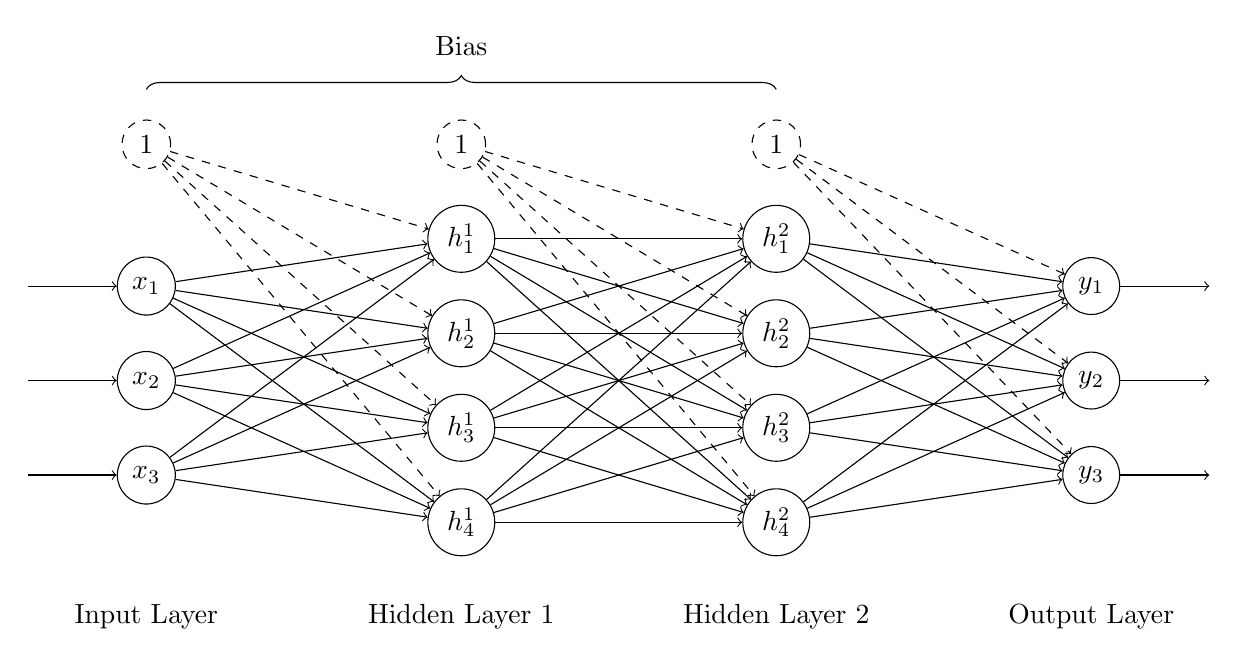
\begin{tikzpicture}
    \tikzstyle{place}=[circle, draw=black, minimum size = 4mm]
    
    % Input
    \draw node [dashed] at (0, 0) [place] (first_0) {$1$};
    \foreach \x in {1,...,3}
      \draw node at (0, -\x*1.2 - 0.6) [place] (first_\x) {$x_\x$};
    \foreach \x in {1,...,3}
      \draw [->] (-1.5, -\x*1.2 - 0.6) to (first_\x); 
    
    % Hidden 1
    \draw node [dashed] at (4, 0) [place] (second_0) {$1$};
    \foreach \x in {1,...,4}
      \node at (4, -\x*1.2) [place] (second_\x) {$h^{1}_\x$};

    % Hidden 2
    \draw node [dashed] at (8, 0) [place] (third_0) {$1$};
    \foreach \x in {1,...,4}
      \node at (8, -\x*1.2) [place] (third_\x) {$h^{2}_\x$};
    
    % Output
    \foreach \x in {1,...,3}
      \node at (12, -\x*1.2 - 0.6) [place] (fourth_\x) {$y_\x$};
    \foreach \x in {1,...,3}
      \draw [->] (fourth_\x) to (13.5, -\x*1.2 - 0.6); 

    \draw [decorate,decoration={brace,amplitude=5pt,raise=-2ex}]
      (0,1) -- (8,1) node[above,midway]{Bias};
      
    % Input -> Hidden 1
    \foreach \i in {1,...,4}
      \draw [->,dashed] (first_0) to (second_\i);
    \foreach \i in {1,...,3}
      \foreach \j in {1,...,4}
        \draw [->] (first_\i) to (second_\j);
    
    % Input -> Hidden 2
    \foreach \i in {1,...,4}
      \draw [->,dashed] (second_0) to (third_\i);
    \foreach \i in {1,...,4}
      \foreach \j in {1,...,4}
        \draw [->] (second_\i) to (third_\j);
    
    % Hidden -> Output
    \foreach \i in {1,...,3}
      \draw [->,dashed] (third_0) to (fourth_\i);
    \foreach \i in {1,...,4}
      \foreach \j in {1,...,3}
        \draw [->] (third_\i) to (fourth_\j);
    
    % Text
    \node at (0, -6) [black, ] {Input Layer};
    \node at (4, -6) [black, ] {Hidden Layer 1};
    \node at (8, -6) [black, ] {Hidden Layer 2};
    \node at (12, -6) [black, ] {Output Layer};
  \end{tikzpicture}}
      \caption{Illustration of a 4-layer multilayer perceptron}
      \label{fig:illustration_deep_network}
  \end{center}
\end{figure}
 
The reason for multi-layers neural networks is that they can model more \textbf{complex non-linear relationships}
~\cite{Goodfellow-et-al-2016} than single 
neurons and single-layer models are able to. Using non-linear activation functions such as ReLU \eqref{eq:relu} allow neurons to model simple 
non-linear functions, and combining these into layers allows them to model these more complex non-linear relationships.

I will denote the function computed by a neural network as $f_{\vec{\theta}}(\vec{x})$, where $\vec{\theta}$ denotes the
weights of the neural network.

\subsection{Neural networks for classification}

A dataset for classification training is given as pairs of numerical \textbf{features} and a \textbf{label}: $(\vec{x}, y)$. These features are 
the input to the network,
and the label is the target. Labels cannot be directly utilised by a neural network as they operate on numerical data. Therefore it is 
necessary to transform the labels into a numerical representation.

\textbf{One-hot encoding} assigns an integer $i$ to each class and makes a vector of length $n$ (where $n$ is the 
number of classes), setting the $ith$ element to one and all other elements to zero. E.g., with three classes
the one-hot labels would be $[1, 0, 0]$ , $[0, 1, 0]$ and $[0, 0, 1]$. The network then has an output node corresponding to each class 
\cite{WhyOneHo55:online}.

The \textbf{softmax} function is then applied to the output of the network to give a probability distribution over the classes. It has the 
form below for each output node $i$, and ensures that the sum of all the output values is one.
\begin{align}
  \sigma(z)_{i} = \frac{e^{i}}{\sum_{k} e^{k}}
\end{align}
A single label can be returned by taking the index of the maximum value in the ouput and correlating that to the label index. 

The \textbf{loss} of the network is the difference between the output of the network and the correct label. The loss should be high 
when the network is performing poorly, and low when it is performing well. For classification the loss function used is the cross 
entropy loss, computed as:
\begin{align}
  J(\vec{\theta}) = - \vec{y} \cdot \log{f_{\vec{\theta}}(\vec{x})} \label{eq:ce}
\end{align}
This is high when the probability of the correct label is low, because $\lim_{x \to 0} -\log{x} = \infty$.

\subsection{Training the network} \label{train}

Neural networks have their weights randomly initialised, and training a neural network involves adjusting them 
($\vec{\theta}$) until the network reaches an acceptable loss or accuracy. This is done by computing 
the gradients of the weights with respect to the loss, and updating the parameters to move the loss towards 
a minimum.

\subsubsection{Updating the weights}

Forward propagation is the flow of information through the network from input features to output values. From these output values the loss is calculated. 
The weights of a neural network can then be updated by first finding the gradient of the loss with respect to these weights.
The process of computing these gradients is called \textbf{backpropagation} and a full derivation can be found in Appendix~\ref{backprop}. The important notation is:

\begin{itemize}
  \item $\theta$ is a vector of all the weights in the network
  \item $J(\vec{\theta})_k$ is the loss for the $kth$ sample in the training set
  \item $\nabla_{\vec{\theta}} J(\vec{\theta})_k$ is a vector of gradients of the loss with respect to all the weights 
\end{itemize}

Once the gradients for all the weights have been calculated the weights are updated. By moving the weights incrementally in the direction of steepest 
negative gradient the loss should decrease as the parameters are shifting it towards a minimum. The model thus gets
better at modelling the training set. These incremental steps are called \textbf{gradient descent}. The weight update rule is: 
\begin{align}
  \vec{\theta} & := \mathbf{\vec{\theta}} - \eta \sum_{k} \frac{\partial J(\vec{\theta})_k}{\partial \mathbf{\vec{\theta}}} \\
  & := \mathbf{\vec{\theta}} - \eta \sum_{k} \nabla_{\vec{\theta}} J(\vec{\theta})_k \\
  & := \mathbf{\vec{\theta}} - \eta \nabla_{\vec{\theta}} \sum_{k} J(\vec{\theta})_k \label{eq:weight}
\end{align}

$\eta$ is a \textbf{hyperparameter}. Hyperparameters are parameters of the model that are not trained but are set by the user before training.
$\eta$ is called the \textbf{learning rate} and controls the size of the step taken each time the weight is updated. If the learning rate is 
too high the weights can ``jump'' over minima, and even diverge out of a minimum, but if the rate is too low it can take too long to converge,
or get stuck in a less desirable local minima. The step size is proportional to the magnitude of the gradient, allowing the optimizer to 
take a larger step towards a minimum if the gradient is steeper.

\subsubsection{Batch learning} \label{batch}

A neural network is generally run over a fixed number of samples for each iteration. This is called 
mini-batch gradient descent and it is the most popular because it has stability advantages over stochastic gradient descent (one sample at a time),
and computational advantages over batch (the entire dataset every iteration). 
Stochastic gradient descent has more noise as each update is based on an individual example, causing the weights to jump around more. It also doesn't take advantage of the 
parallelisation possiblity of GPUs - it's much more efficient to send multiple samples through at once. Batch has the problem of storing the whole 
dataset in memory, and only making one update per pass through the dataset can mean the model takes longer to converge to the best parameters. Mini-batch manages to
have less noise than stochastic due to averaging over multiple samples, while also taking advantage of parallelisation and not requiring huge amounts of memory.

\subsubsection{Summary}

One complete pass through the dataset 
is called an \textbf{epoch} and 
training involves running forward and backpropagation for a certain number of epochs to minimise the loss
on the training set and cause the model to converge to a good approximation to the real function. The pseudocode for training the network 
is shown below.
\begin{algorithm}
  \begin{algorithmic}[1]
    \Procedure{Training}{$i$, $\mathcal{D}$, $\eta$, \texttt{model}, \texttt{loss\char`_function}}
    \For{$i$ epochs}
    \For{mini-batch $\mathcal{M}$ in $\mathcal{D}$}
    \State \texttt{data, labels} = $\mathcal{M}$
    \State \texttt{out} = \texttt{model(data)}
    \State $\mathcal{J}$ = \texttt{loss\char`_function(out, labels)}
    \State \texttt{model}.$\vec{\theta}$ = \texttt{model}.$\vec{\theta}$ - $\eta \nabla_{\vec{\theta}} \mathcal{J}$ 
    \EndFor
    \EndFor
    \EndProcedure
  \end{algorithmic}
  \caption{Train neural network via mini-batch gradient descent} 
  \label{alg:train}
\end{algorithm}

\section{The manifold hypothesis}

\textbf{Dimensionality} refers to the number of features needed to specify data. For example, a very popular machine learning dataset
is MNIST, containing 28x28 grayscale images of handwritten digits. The dimensionality of each datapoint is 784, as that is the
number of pixels specifying each image.

\textbf{The manifold hypothesis} suggests that high-dimensional data can actually be viewed as lying on or near to a
lower-dimensional manifold embedded in this higher-dimensional space.

The definition of an n-dimensional manifold is ``a 
topological space that is locally Euclidean'', i.e. there is a neighbourhood around each point on the manifold that can be describe as n-dimensional 
Euclidean space. It is much easier to grasp with an intuitive example - imagine that all the datapoints in a 
dataset lie on piece of paper, and so can be described with two features, an $x$ and $y$ axis. If the paper is scrunched up 
it now has a three dimensional shape, but the data still lies on a two-dimensional manifold. Unscrunch the paper and it can still 
be described with only two features.
\begin{figure}[H]
  \centering
  \includegraphics[scale=.75]{figs/manifold.png}
  \caption{Points on a 2-dimensional manifold embedded in 3-dimensional space}
  \label{fig:manifold}
\end{figure}

The manifold hypothesis suggests that many features in high-dimensional data are actually redundant,
i.e. it can be described using fewer features. Again this can be seen intuitively in that the set of 784 pixel images 
that look like a recognisable digit is a very small subset of 784 pixel images - randomly selected pixel values look like 
random noise, suggesting that there is a lot of redundancy in the MNIST features.
\begin{figure}[H]
  \centering
  \begin{subfigure}[b]{0.4\linewidth}
    \centering
    \includegraphics[scale=.25]{figs/rand_noise.pdf}
    \caption{Pixel values selected randomly}
  \end{subfigure}
  \begin{subfigure}[b]{0.4\linewidth}
    \centering
    \includegraphics[scale=.25]{figs/digit.pdf}
    \caption{MNIST digit}
  \end{subfigure}
  \caption{Demonstrating redundancy of features in MNIST dataset}
  \label{fig:digit}
\end{figure}

This leads to \textbf{non-linear dimensionality-reduction} techniques. By finding this lower-dimensional
manifold the data can be explained with fewer features and possibly be more easily separated and classified. Going back to the paper example,
linear-dimensionality reduction techniques would be able to find the 2D embedding if the paper were 
rotated, translated or stretched, but would be unable to unscrunch the paper, as that is a non-linear transformation. Autoencoders are 
used for non-linear dimensionality reduction, and are described in the next section.

\section{Autoencoders}

Autoencoders use neural networks in an unsupervised way to learn new \textbf{latent} representations of data, typically with reduced 
dimensionality (i.e. there are fewer features in the latent data than in the input data). The use of neural networks allow the autoencoder 
to learn a non-linear mapping from the data to the latent representation.

Autoencoders compromise an encoder and a decoder. The encoder takes in the original data, $\vec{x}$, 
and outputs a latent representation, $\vec{z} = f_{\vec{\theta}}(\vec{x})$. The decoder then takes this latent representation and 
attempts to reconstruct $\vec{x}$, outputting $\vec{\hat{x}} = h_{\vec{\phi}}(\vec{z})$. This allows an unsupervised problem to be turned 
into a supervised problem, using $\vec{x}$ as the target.
\begin{figure}[H]
  \begin{center}
      \scalebox{.75}{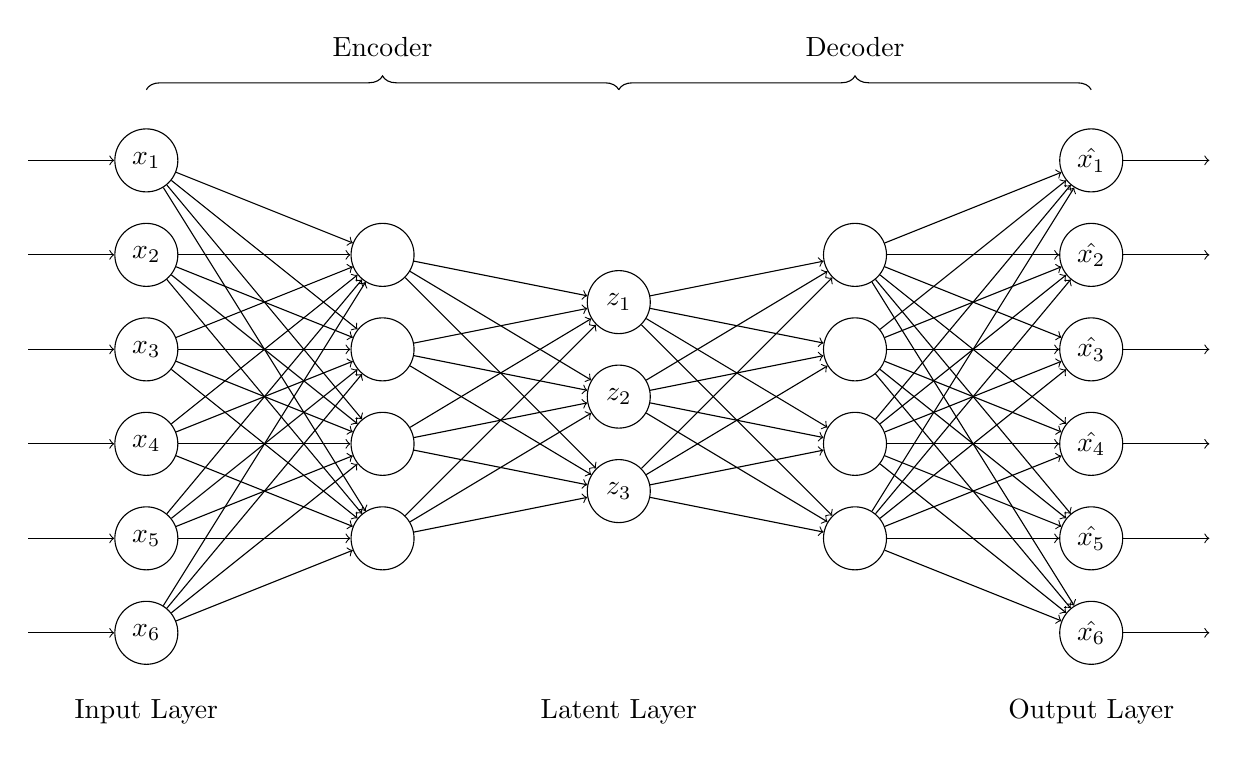
\begin{tikzpicture}
    \tikzstyle{place}=[circle, draw=black, minimum size = 8mm]

    % Input
    \foreach \x in {1,...,6}
        \draw node at (0, -\x*1.2) [place] (first_\x) {$x_\x$};

    % Hidden 1
    \foreach \x in {1,...,4}
        \node at (3, -1.2 -\x*1.2) [place] (second_\x){};

    % Latent
    \foreach \x in {1,...,3}
        \node at (6, -1.8 -\x*1.2) [place] (third_\x){$z_\x$};

    % Hidden 2
    \foreach \x in {1,...,4}
        \node at (9, -1.2 -\x*1.2) [place] (fourth_\x){};

    % Output
    \foreach \x in {1,...,6}
        \draw node at (12, -\x*1.2) [place] (fifth_\x) {$\hat{x_\x}$};
        
    \foreach \i in {1,...,6}
        \draw [->] (-1.5, -\i*1.2) to (first_\i);

    \foreach \i in {1,...,6}
        \foreach \j in {1,...,4}
        \draw [->] (first_\i) to (second_\j);

    \foreach \i in {1,...,4}
        \foreach \j in {1,...,3}
            \draw [->] (second_\i) to (third_\j);

    \foreach \i in {1,...,3}
        \foreach \j in {1,...,4}
        \draw [->] (third_\i) to (fourth_\j);

    \foreach \i in {1,...,4}
        \foreach \j in {1,...,6}
            \draw [->] (fourth_\i) to (fifth_\j);

    \foreach \i in {1,...,6}
        \draw [->] (fifth_\i) to (13.5, -\i*1.2);

    \draw [decorate,decoration={brace,amplitude=5pt,raise=-2ex}]
        (0,0) -- (6,0) node[above,midway]{Encoder};
    \draw [decorate,decoration={brace,amplitude=5pt,raise=-2ex}]
        (6,0) -- (12,0) node[above,midway]{Decoder};

    % Text
    \node at (0, -8.2) [black, ] {Input Layer};
    \node at (6, -8.2) [black, ] {Latent Layer};
    \node at (12, -8.2) [black, ] {Output Layer};
\end{tikzpicture}}
      \caption{Illustration of a simple autoencoder}
      \label{fig:illustration_autoencoder}
  \end{center}
\end{figure}

\subsection{Simple autoencoders}

Simple autoencoders constrain the network by making the number of latent features smaller than the number of input
features. This prevents the network from simply learning the identity function, and hopefully results in an informative latent space.

\subsubsection{Training}
Autoencoders can be trained end to end using backpropagation as explained in Section \ref{train}. The target $\vec{x}$ and output 
$\vec{\hat{x}}$ are both vectors and so 
the \textbf{squared Euclidean distance}\footnote{also known as mean square error} is used as the loss per datapoint. Both the encoder weights 
$\vec{\theta}$ and 
decoder weights $\vec{\phi}$ 
are trained at the 
same time; the gradients are backpropagated through the decoder to the latent layer and then back through the encoder. 

\subsection{Denoising autoencoders}

Denoising autoencoders corrupt the input data with noise (e.g. by adding Gaussian noise) giving $\tilde{\vec{x}}$, which is then used as the 
input to the network. However, the target is the uncorrupted input data, 
$\vec{x}$. The aim is to force the autoencoder to learn a better set of features because it not only has to reconstruct the data but also 
has to remove the noise. They can be trained in the same way as a simple autoencoder.

\subsection{Variational autoencoders} \label{vae}

Variational autoencoders were 
introduced by Kingma and Welling in 2013~\cite{DBLP:journals/corr/KingmaW13} and have become one of the most popular unsupervised learning techniques. 
They are based on Bayesian inference, and differ from other autoencoders in that the encoder outputs
the parameters of a probability distribution over the latent variables, rather than a single configuration.
\begin{figure}[H]
  \begin{center}
      \scalebox{.75}{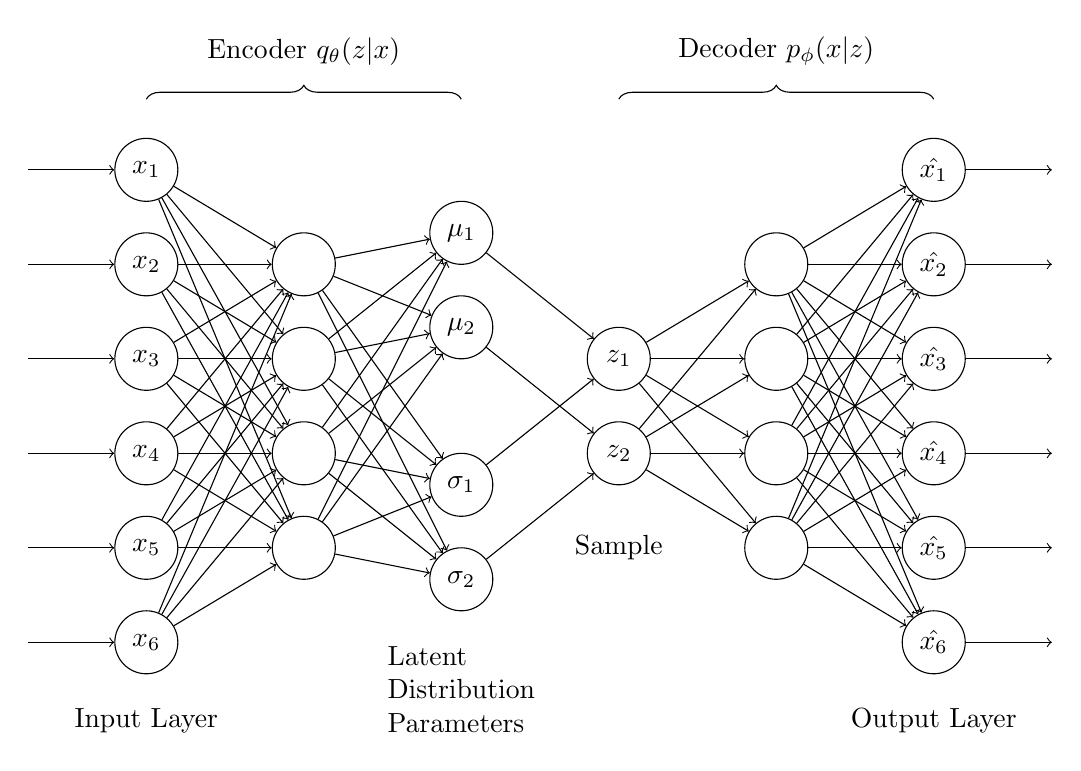
\begin{tikzpicture}
    \tikzstyle{place}=[circle, draw=black, minimum size = 8mm]
    
    % Input
    \foreach \x in {1,...,6}
        \draw node at (0, -\x*1.2) [place] (first_\x) {$x_\x$};
    
    % Hidden 1
    \foreach \x in {1,...,4}
        \node at (2, -1.2 -\x*1.2) [place] (second_\x){};

    % Mu
    \foreach \x in {1,...,2}
        \node at (4, -0.8 -\x*1.2) [place] (mu_\x){$\mu_\x$};

    \foreach \x in {1,...,2}
        \node at (4, -4 -\x*1.2) [place] (logvar_\x){$\sigma_\x$};

    \foreach \x in {1,...,2}
        \draw node at (6, -2.4 -\x*1.2) [place] (sample_\x){$z_\x$};

    % Hidden 2
    \foreach \x in {1,...,4}
        \node at (8, -1.2 -\x*1.2) [place] (fourth_\x){};
    
    % Output
    \foreach \x in {1,...,6}
        \draw node at (10, -\x*1.2) [place] (fifth_\x) {$\hat{x_\x}$};
        
    \foreach \i in {1,...,6}
        \draw [->] (-1.5, -\i*1.2) to (first_\i);

    \foreach \i in {1,...,6}
        \foreach \j in {1,...,4}
        \draw [->] (first_\i) to (second_\j);

    \foreach \i in {1,...,4}
        \foreach \j in {1,...,2}
            \draw [->] (second_\i) to (mu_\j);
    \foreach \i in {1,...,4}
        \foreach \j in {1,...,2}
        \draw [->] (second_\i) to (logvar_\j);

    \foreach \i in {1,...,2}
        \draw [->] (logvar_\i) to (sample_\i);
    
    \foreach \i in {1,...,2}
        \draw [->] (mu_\i) to (sample_\i);

    \foreach \i in {1,...,2}
        \foreach \j in {1,...,4}
        \draw [->] (sample_\i) to (fourth_\j);
    
    \foreach \i in {1,...,4}
        \foreach \j in {1,...,6}
        \draw [->] (fourth_\i) to (fifth_\j);

    \foreach \i in {1,...,6}
        \draw [->] (fifth_\i) to (11.5, -\i*1.2);

    \draw [decorate,decoration={brace,amplitude=5pt,raise=-2ex}]
        (0,0) -- (4,0) node[above,midway]{Encoder $q_\theta(z|x)$};
    \draw [decorate,decoration={brace,amplitude=5pt,raise=-2ex}]
        (6,0) -- (10,0) node[above,midway]{Decoder $p_\phi(x|z)$};
    
    % Text
    \node at (0, -8.2) [black, ] {Input Layer};
    \node at (4, -7.8) [black, align=left] {Latent \\ Distribution\\ Parameters};
    \node at (6, -6) [black, ] {Sample};
    \node at (10, -8.2) [black, ] {Output Layer};
\end{tikzpicture}}
      \caption{Illustration of a Gaussian variational autoencoder}
      \label{fig:gauss_vae}
  \end{center}
\end{figure}

The central idea of variational autoencoders is that the data $\vec{x}$ has been generated from some lower-dimensional latent
representation $\vec{z}$. The latent distribution describes the variation in the data, and so these are called 
\textbf{latent variable models}. Each datapoint $\vec{x_{i}}$ is generated by:
\begin{itemize}
  \item sampling $\vec{z_{i}}$ from the prior distribution over $\vec{z}$: $\vec{z_{i}} \sim p(\vec{z})$, 
  \item sampling $\vec{x_{i}}$ from the conditional distribution $p(\vec{x}|\vec{z})$ (known as the likelihood): \\ 
  $\vec{x_{i}} \sim p(\vec{x}|\vec{z}=\vec{z_{i}})$
\end{itemize}

The prior $p(\vec{z})$ can be thought of as constraining the possible space of latent variables. In an unconstrained latent space, a
normal autoencoder could place the same character written in different styles in different areas of n-dimensional Euclidean space (where n is the 
dimensionality of $z$) as the latent representation is a vector of unconstrained real numbers. This is detrimental to learning a meaningful 
latent space, and by constraining this space with a prior it should force the model to keep the representations of similar datapoints close~\cite{Tutorial70:online}.

The decoder of the VAE is a neural network that models the likelihood represented as $p_{\vec{\phi}}(\vec{x}|\vec{z})$. Once the VAE is 
trained, new samples similar to 
those in the training set can be generated by sampling from the prior and passing this into the decoder; this is why VAEs are often
referred to as generative models.

In most situations where unsupervised learning is useful, only $\vec{x}$ is known. The goal is then to infer $\vec{z}$.
Inference in the model refers to finding good values of the latent variables given the data. This can be done by computing the
posterior, $p(\vec{z}|\vec{x})$. Using Bayes' rule we have:
\begin{equation}
  p(z|x) = \frac{p(x|z)p(z)}{p(x)}
\end{equation}

The denominator $p(\vec{x})$ is known as the evidence, and calculating it is intractable as it has to be computed by marginalizing out $\vec{z}$:
\begin{equation}
  p(x) = \int p(x|z)p(z) dz
\end{equation}

Computing this integral requires exponential time as it has to be computed over all the possible configurations of
the latent variables. Therefore the posterior is approximated using a neural network $q_{\vec{\theta}}(\vec{z}|\vec{x})$. 
This is the encoder.

\subsubsection{Training}

The loss function used for a variational autoencoder can be derived by maximizing the probability of the evidence.
This makes sense intuitively, as a good model should maximise the probability of the real data~\cite{SVIPartI90:online}. A full derivation
of this loss can be found in Appendix~\ref{vae_loss}, but the final form is below:
\begingroup
\allowdisplaybreaks
\begin{align}
  \log p(x) = \mathbb{E}_q [\log p(x|z)] - D_{KL}(q(z|x)||p(z))
\end{align}
\endgroup

This is the \textbf{evidence lower bound} (ELBO). Maximizing the ELBO maximizes the probability of the 
evidence in the model, meaning the model fits the data as well as possible. The two terms in the ELBO correspond to the negative 
reconstruction loss (squared Euclidean distance) between the input and output, and the \textbf{Kullback-Leibler divergence} (KLD) between 
the computed posterior and the prior distribution of the latent variables. 
The KLD measures the difference between two probability distributions, and this acts as a regularizing term, constraining the distribution 
of the latent variables to be close to the prior. Taking the 
negative of the ELBO gives the loss function for the variational autoencoder. Minimizing this loss function is equivalent to maximising the ELBO.

\paragraph{The Gaussian VAE}is the most common and the one used in this project. The prior $p(\vec{z})$ is chosen to be the standard Gaussian, 
$\mathcal{N}(0, 1)$,
for every latent variable. The output from the encoder is a vector of means $\vec{\mu}$ and standard deviations $\vec{\sigma}$ of normal distributions. 
During training, data is fed in mini-batches into the encoder and latent variables are then sampled from the encoder output: 
$\vec{z_{i}} \sim \mathcal{N}(\vec{\mu}, \vec{\sigma}^{2})$. These are fed into the decoder which outputs a reconstruction $\vec{\hat{x}}$. 
The loss for each datapoint is then computed as the reconstruction loss between $\vec{\hat{x}}$ and $\vec{x}$ and the KLD between
$\mathcal{N}(\vec{\mu}, \vec{\sigma}^{2})$ and $\mathcal{N}(0, 1)$.

Training is again done by backpropagation but
it is not possible to backpropagate the reconstruction loss through the drawing of the random sample, and so 
\textbf{the reparameterization trick} is used. 
An explanation can be found in Appendix ~\ref{reparam}.

\section{Semi-supervised models} \label{ss_models}

Semi-supervised learning involves leveraging large amounts of unlabelled data to increase model performance on supervised learning tasks. 
In most fields, unlabelled data is much easier to obtain than labelled data. I noted in the Introduction that wealth of gene 
expression data for many different organisms is available online, albeit that the phenotype a researcher wants 
to study is often not included. With standard supervised learning this data is unusable, but semi-supervised learning
can use it to improve performance. 

\subsection{Dimensionality reduction (M1)} \label{m1}

The simplest semi-supervised model in this project relies on the manifold hypothesis. It uses a variational autoencoder to construct a
reduced dimensionality feature representation of the data that should cluster similar samples together, and is partially based 
on the Kingma M1 model~\cite{DBLP:journals/corr/KingmaRMW14}. The idea is that it should then be 
easier to classify the datapoints in this latent dimension, even with a limited amount of labelled data.

\subsection{Network pre-training} \label{sdae}

\textbf{Stacked denoising autoencoders} are a way of pre-training deep networks one layer at a time, using unlabelled data. 
Each hidden layer in the network is 
trained as part of a one-layer denoising autoencoder, with the layer to be trained used as the encoder and a new temporary layer constructed
as the decoder. The autoencoder takes the ouput from the previous layer in the network and uses this as the input, injecting noise before 
passing it through the autoencoder and attempting to reconstruct the clean input. The reconstruction loss is then backpropagated through 
the autoencoder only (no other layers of the deep network) and the weights are updated. The loss computed by the autoencoder is referred to 
as an unsupervised ``local denoising criterion''~\cite{Vincent:2010:SDA:1756006.1953039} as it does not require a label and is computed only 
for one layer at a time rather than the whole network.

The network is trained one layer at a time, beginning with the first hidden layer. Once the reconstruction loss for the denoising autoencoder has 
converged for the layer, the decoder is discarded, and the next layer is trained in the same way, using the output of the previously trained
layer as input.

Once this unsupervised pre-training is finished the model is then \textit{fine-tuned} by running normal supervised training, backpropagating
classification loss through the entire network and updating the weights.

Unsupervised pre-training with a stacked denoising autoencoder provides a good prior to the supervised training.
The pre-training procedure provides an initialization point for the supervised training where the parameters are restricted, hopefully to an area 
closer to the global minimum for the loss function~\cite{Erhan:2010:WUP:1756006.1756025}.

\subsection{The semi-supervised VAE (M2)} \label{ssVAE}

The semi-supervised VAE is a model introduced by Kingma et al.~\cite{DBLP:journals/corr/KingmaRMW14} that extends the VAE to include label information. 
The assumption used is that the data $\vec{x}$ is generated from both a discrete label $y$ and a continuous latent representation 
$\vec{z}$, which are marginally independent of each other.
Therefore $y$ encodes the class of the data, while $\vec{z}$ encodes everything else. In the MNIST dataset this means that $y$ encodes
what digit the character is, while $\vec{z}$ encodes the style. The generative model (the decoder) works by sampling $y$ from a 
categorical distribution $p(y)$ and by sampling $\vec{z}$ from a continuous distribution $p(\vec{z})$ (usually a Gaussian), before computing 
$p(\vec{x}|y, \vec{z})$ using a neural network $p_{\vec{\phi}}(\vec{x}|y, \vec{z})$.
\begin{figure}[H]
  \begin{subfigure}[b]{0.5\textwidth}
    \centering
    \scalebox{.9}{\begin{tikzpicture}
    \draw node at (0, 0) [place] (z) {$\vec{z}$};
    \draw node at (2, 0) [place] (y) {$\vec{y}$};
    \draw node at (1, -2) [place] (x) {$\vec{x}$};

    \begin{scope}[on background layer]
    \fill[fill=gray!25] (x.0) arc [start angle=0, end angle=360, radius=4mm];
    \fill[fill=gray!25] (y.270) arc [start angle=270, end angle=450, radius=4mm];
    \end{scope}

    \draw [->] (z) to (x);
    \draw [->] (y) to (x);
\end{tikzpicture}}
    \caption{The generative model}
  \end{subfigure}
  \begin{subfigure}[b]{0.5\textwidth}
    \centering
    \scalebox{.9}{\input{figs/inference.tex}}
    \caption{The inference model}
  \end{subfigure}
  \caption[Semi-supervised VAE]{The semi-supervised VAE \\ (shading indicates that a variable in the dataset is observed)}
  \label{fig:ss_vae}
\end{figure}

In the semi-supervised model there are two inference cases. When the data is labelled the question is how to infer $\vec{z}$ from $\vec{x}$ and $y$.
Both $\vec{x}$ and $\vec{y}$ are used as input to the encoder, while $y$ and $\vec{z}$ are used as input to the decoder.
This helps the encoder to learn to separate the representation of $y$ and $\vec{z}$, so that $\vec{z}$ contains
no information about the label. The semi-supervised VAE in this project uses a Gaussian distribution as the prior distribution for 
$\vec{z}$ (like the unsupervised VAE), and the encoder models $q(\vec{z}|\vec{x}, y)$ with a network $q_{\theta}(\vec{z}|\vec{x}, y)$. For labelled data 
the model should 
maximise the evidence $p(\vec{x}, y)$, the probability of the real labelled data. This leads to a variant of the ELBO by marginalizing
out $z$:
\begin{align}
  \log p(x, y) & = \mathbb{E}_q [\log p(x|y, z) + \log p(y)] - D_{KL}(q(z|x, y)||p(z)) \\
  & = -\mathcal{L}(x, y)
\end{align}

The derivation is not included in the Kingma paper~\cite{DBLP:journals/corr/KingmaRMW14}, which includes only the line above and so I had 
to derive it myself. The derivation can be found in Appendix~\ref{ssvae_loss}.

It is very similar to the ELBO for the normal VAE, except that there is now a prior over $y$. This encodes previous knowledge about the 
distribution of the classes $y$, penalizing the model more when the label is of a low probability class. This is unimportant for the labelled
data as the previous knowledge is drawn from this data, but becomes important for the unlabelled data, and the connection between the two can be 
seen in the unlabelled ELBO below. A good model maximises the ELBO and therefore minimises $\mathcal{L}(x, y)$, which is used as the loss function.

When the data is unlabelled, the problem is of inferring both $y$ and $\vec{z}$ from $\vec{x}$, $q(y, \vec{z}|\vec{x})$. The evidence in the unlabelled 
case is $p(\vec{x})$,
and the ELBO can be derived by marginalizing out both $y$ and $\vec{z}$:
\begin{align}
  \log p(x) & = \sum_{y} q(y|x)(-\mathcal{L}(x, y)) + \mathcal{H}(q(y|x)) \\
  & = -\mathcal{U}(x, y)
\end{align}
This derivation is also in Appendix~\ref{ssvae_loss}.

The marginalization of $y$ is done by summation because the labels are discrete. Looking at the penultimate line of the derivation there is
the term $q(y|x)$. This is classification, inferring $y$ from $\vec{x}$. This classifier is parameterised
by a neural network, and outputs a categorical distribution over the labels.

The summation term is referred to as ``classification as inference'' by Kingma~\cite{DBLP:journals/corr/KingmaRMW14}. For each label the labelled loss with 
respect to the data and that label is calculated and then multiplied by the probability of the label. This means that if a particular label
leads to a bad reconstruction (implying that the label was incorrect) and the classifier assigns a high probability to that label, 
the loss to the classifier will be very high, and minimizing this loss should lead to better classification. The prior over $y$ in $\mathcal{L}(x, y)$
becomes important here as it discourages the classifier from assigning a high probability to an unlikely class. All of this means that 
the classifier can learn directly from unlabelled data, with the small amount of labelled data providing a guide to good reconstructions.

The pipelines for labelled and unlabelled data are slightly different. Labelled data is fed directly into the encoder
along with its label, and the loss function $\mathcal{L}(x, y)$ is calculated and backpropagated through the network. Unlabelled data is 
first put through the classifier, before it is fed into the encoder once with each label allowing $\mathcal{U}(x)$ to be computed and 
backpropagated through the network.

Currently at no point does the classifier learn directly from the labelled data, inhibiting the model. To remedy
this the labelled loss function is modified to include an extra term, the cross entropy loss~\eqref{eq:ce} between the real label and the 
label the classifier outputs for the data. This modified version is then:
\begin{align}
  \mathcal{J}(x, y) = \mathcal{L}(x, y) - \alpha (y \cdot \log q(y|x))
\end{align}

$\alpha$ is a hyperparameter that controls the weighting of the supervised loss, and is configured depending on the amount of labelled and 
unlabelled data available.

The model can now learn to classify from both labelled and unlabelled data at the same time, and so does not require pretraining as
the previous models did.

\subsection{The ladder network} \label{ladder}

The ladder network is the most recent of the models included in this project, having first been described by Valpola in 2014
~\cite{DBLP:journals/corr/Valpola14}, and then expanded upon by Rasmus et al. in 2015~\cite{DBLP:journals/corr/RasmusVHBR15}. 
It has some similarity to the SDAE, using an unsupervised local denoising criterion, but the structure of the model is very different.
The model is made up of an encoder and decoder, like an autoencoder, but with lateral connections between the layers in the encoder 
and decoder. The final classifier is the encoder.

\begin{figure}[H]
  \centering
  \includegraphics[scale=0.4]{figs/ladder.png}
  \caption[Illustration of the ladder network]{Illustration of the ladder network \\ (Source: Rasmus et al.~\cite{DBLP:journals/corr/RasmusVHBR15})}
  \label{fig:ladder}
\end{figure}

The ladder network is a hierarchical latent variable model, which differ from the latent variable models
looked at so far in that it attempts to represent the data using multiple layers of latent variables, rather than a 
single layer. 
In the normal autoencoder or VAE the single latent layer $\vec{z}$ has to encode everything about the data $\vec{x}$, otherwise the reconstruction it generates 
will be very poor. With a hierarchical model each layer models only some information about $\vec{x}$, with the higher layers able to be 
more abstract, 
as they don't have to model the details encoded in the lower layers. 

For example, using MNIST, $\vec{z}$ in an
autoencoder cannot just be the digit label as this does not provide enough information to reconstruct the original image well. 
In a hierarchical latent variable model the highest
level latent variable is able to be very abstract and only encode the label, as the other layers in the model provide less abstract 
information (e.g about style and location) that can lead to a good reconstruction.

The reason this works in the ladder network is because the lateral connections``leak'' information from layers in the encoder to the decoder. 
This means that each decoder layer
receives information both from the previous decoder layer and the corresponding encoder layer. The encoder layer passes some information which
the subsequent encoder layers then no longer have to model, as the decoder will receive it directly from the encoder layer.

This structure, with the representation becoming more abstract in higher level layers, is also analagous to how supervised learning works, with the layers 
further into the network modelling more complicated and abstract features, and with the final layer just outputting a class label.

The way these lateral connections work is that
at the input to each decoder layer $\vec{u}^{(l)}$ the corresponding encoder representation $\vec{z}^{(l)}$ and the output of the previous decoder layer $\vec{u}^{(l+1)}$ are combined
using a combinator function $g$. $g$ has trainable parameters (weights), but this leads to a problem where the lowest possible unsupervised loss can be 
achieved by $g$ in the first layer learning to copy $\vec{z}^{(0)}$ and completely ignoring $\vec{u}^{(l+1)}$, which corresponds to copying the input directly to the output at the bottom layer.
This short circuits the autoencoder, and in order to prevent this, Gaussian noise (sampled from $\mathcal{N}(0, 1)$) is added to the input to each layer 
in the encoder. Each encoder layer then has the representation $\vec{\tilde{z}}^{(l)}$ and this noise means that just copying over the input no longer minimises the loss function. 

However, if the unsupervised loss function used is simply the reconstruction loss between the decoder output $\vec{\hat{x}}$ and the encoder input $\vec{x}$, the first layer of 
the network still has a disproportionate
influence on the loss. In order to remedy this Valpola proposes adding a local denoising criterion. This involves adding a cost function at each layer of the decoder,
namely the reconstruction loss between $g(\vec{\tilde{z}}^{(l)}, \vec{u}^{(l+1)})$ (which is $\vec{\hat{z}}^{(l)}$, a denoised representation of $\vec{\tilde{z}}^{(l)}$) and $\vec{z}^{(l)}$, the clean 
representation from layer $l$ of the encoder. In order to generate both the clean and noisy encoder representations, the encoder is run twice per training iteration,
once without the added noise to generate $\vec{z}^{(l)}$, and once with noise to generate $\vec{\tilde{z}}^{(l)}$. These local cost functions require all the layers to learn in order
to make a meaningful representation that can be denoised well. Each layer loss is multiplied by a hyperparameter $\lambda_{l}$ according to how important the denoising cost
of the layer is, before being summed together to give a final unsupervised cost function per sample of:

\begin{align}
  \mathcal{U}(x) = \sum_{l} |z^{(l)} - \hat{z}^{(l)}|^{2}
\end{align}

The model as explained so far allows the ladder network to learn abstract features in the higher layers. However, without supervised data and a supervised loss function the 
features learned are unlikely to be useful for the classification task. The small amount of labelled data is used as a guide for this. The classifier 
is the encoder so the data is passed through the noisy encoder during training (the noise acts as a regularizer~\cite{NoiseInj}) and cross entropy 
loss~\ref{eq:ce} is computed between the output and the labels. When the classifier is used for inference after being trained, no noise is 
added.

An overview of the training process can be found in Section~\ref{ladder_imp}

\section{Requirements analysis}

By taking the success criteria from the project proposal (Appendix ~\ref{proposal}) I constructed a set of tasks that must be completed 
and ranked them by their priority. The success criteria are:

\begin{itemize}
  \item The implemented models achieve close to original paper performance on the MNIST dataset 
  \item The final chosen model achieves better prediction accuracy than supervised learning alone on genetic datasets
  \item A tool is built that takes in file paths to unlabelled and labelled data and trains a classifier based on this
\end{itemize}

The first success criterion differs from the project proposal. After reading the papers of the models to be implemented, I 
realised that the semi-supervised variational autoencoder and the ladder network both had benchmarks given on 
the MNIST database of handwritten digits~\cite{lecun-mnisthandwrittendigit-2010}. As the stated aim of generating synthetic data was to
ensure that the models were working correctly, I decided that a better measure of the correctness of the models was whether they
achieved (close to) the accuracy reported in the papers.

The models compared in this project are those described in the previous section and so, with these models selected and the success criteria 
defined above, the requirements can be constructed:

\begin{table}[H]
  \label{tab:requirements}
  \small % text size of table content
  \centering % center the table
  \begin{tabular}{cc} % alignment of each column data
  \toprule[\heavyrulewidth]\toprule[\heavyrulewidth]
  \textbf{Requirement} & \textbf{Priority} \\ 
  \midrule
  Implement simple multilayer perceptron & Medium \\
  Implement M1 model & Medium \\
  Implement stacked denoising autoencoder & Medium \\
  Implement semi-supervised autoencoder & High \\
  Semi-supervised autoencoder achieves close to original paper \\ accuracy on MNIST & Medium \\
  Implement ladder network & High \\
  Ladder network achieves close to original paper accuracy \\ on MNIST & Medium \\
  Process the Cancer Genome Atlas gene expression data & High \\
  Evaluate and compare performance of models on MNIST & Low \\
  Evaluate and compare performance of models on TCGA data & High \\
  Implement saliency for best performing model (extension) & Low \\
  \bottomrule[\heavyrulewidth] 
  \end{tabular}
  \caption{Requirements for a successful project} 
\end{table}

\section{Starting point and reading} \label{reading}

I had some previous knowledge about neural networks and machine learning techniques through completing \textit{Introduction to data science}
and \textit{Artificial intelligence I} as part of Part IB, and completing the machine learning course by Andrew Ng on Coursera. However,
I had no previous experience with autoencoders and semi-supervised learning, and little experience of optimising 
a machine learning model and Bayesian inference. To this end I decided upon a list of essential reading:~\cite{ML_Bayes}~\cite{Goodfellow-et-al-2016}
~\cite{DBLP:journals/corr/KingmaW13}~\cite{DBLP:journals/corr/KingmaRMW14}~\cite{Vincent:2010:SDA:1756006.1953039}
~\cite{DBLP:journals/corr/Valpola14}~\cite{DBLP:journals/corr/RasmusVHBR15}.

\section{Software engineering}

All the models in this project were developed iteratively. They were first constructed in their most basic form, and tested on MNIST 
data to determine whether they were working correctly. Enhancements such as early stopping and other hyperparameter optimisations were 
added in stages, and the models were tested on MNIST at each stage to ensure that the changes had not led to any problems.

\section{Resources}

\subsection{Language and libraries}
I made the decision to use Python, as it supports the deep learning library PyTorch.  After trying both PyTorch and Tensorflow, 
and looking at a comparison of the features offered, I decided to 
use PyTorch, as it felt more flexible, allowing much easier access 
to intermediate variables for debugging. In Tensorflow all operations have to be run using a Session object, and the only variables a 
user can see are those returned from the session.

I used the PyCharm IDE for writing my Python code as I was familiar with Jetbrains IDEs.
PyCharm includes useful features like autocomplete, and has good integration with \texttt{git}.

\subsection{Hardware}
All of the coding was done on my laptop (2.6 GHz Intel Core i5, 8GB RAM, 128GB SSD).

The models are computationally intensive, and run much 
quicker on a GPU. To this end I was given access to NVIDIA P100 GPUs on the Cambridge HPC by Prof. Li\'o.

\subsection{Backing up}
To back up my project and dissertation files and code I stored them in a \texttt{git} repository synced with a remote repository on GitHub. I also 
made regular backups of my entire SSD to an external hard drive.

\section{Summary}
This section should have provided an overview of the theory behind this project, and of the requirements that must be completed to 
ensure the project is a success.